\subsection{Transfer to image classification}
Efficient transfer learning with large scale backbones is often achieved by using them as frozen feature extractors. This section presents the evaluation results of \chonk for image classification using linear probing and locked-image tuning as well as out-of-distribution transfer. Additional results for  Head2Toe transfer, few-shot transfer, and linear probing with L-BFGS can be found in \cref{app:image_classification}.

\subsubsection{Linear probing}

% We perform linear probing of the pre-logits (the representation after the pooling by MAP head) transfer to both ImageNet-1k as a standard benchmark, as well as iNaturalist~\citep{cui2018large} for benchmarking linear separability of fine-grained concepts.

We explored various ways of training a linear probe, % we defer the details to Appendix~\ref{app:linear}.
our final setup on ImageNet uses SGD with momentum for 10 epochs at 224px resolution, with mild random cropping and horizontal flipping as the only data augmentations, and no further regularizations.
% (no L2 penalty).
% Isn't it clear that there's no l2? We can add it if amigious


The results presented in \cref{tab:linear_probe_i1k} show that while the returns are diminishing, there is still a notable improvement at this scale\footnote{We repeated a subset of the experiments multiple times and the results are almost identical.}.
Furthermore, we show that linear probing of larger models like \chonk can approach or exceed performance of full fine-tuning of smaller models with high-resolution, which can be often cheaper or easier to do.


% Data from go/lb-linear
\begin{table}[ht]
    \caption{Linear evaluation on ImageNet-1k~\citep{deng2009imagenet} with varying scale. All models pre-trained on large datasets. 
    Performances of a few high-resolution fine-tuned models from are provided for reference.}
    \centering
    \setlength{\tabcolsep}{4pt}
    \resizebox{.6\columnwidth}{!}{%
    \begin{tabular}{@{} l l c c c c c @{}}
        \toprule
        Model & IN & ReaL & INv2 & ObjectNet & IN-R & IN-A \\
        \midrule
        \multicolumn{7}{l}{\textit{224px linear probe (frozen)}} \\
        \midrule
        B/32 & 80.18 & 86.00 & 69.56 & 46.03 & 75.03 & 31.2 \\
        B/16 & 84.20 & 88.79 & 75.07 & 56.01 & 82.50 & 52.67 \\
        ALIGN (360px) & 85.5 & - & - & - & - & - \\
        L/16 & 86.66 & 90.05 & 78.57 & 63.84 & 89.92 & 67.96 \\
        g/14 & 88.51 & 90.50 & 81.10 & 68.84 & 92.33 & 77.51 \\
        G/14 & 88.98 & 90.60 & 81.32 & 69.55 & 91.74 & 78.79 \\
        e/14 & 89.26 & 90.74 & 82.51 & 71.54 & \textbf{94.33} & 81.56 \\
        22B  & \textbf{89.51} & \textbf{90.94} & \textbf{83.15} & \textbf{74.30} & 94.27 & \textbf{83.80} \\
        \midrule
        \multicolumn{7}{l}{\textit{High-res fine-tuning}} \\
        \midrule
        L/16 & 88.5 & 90.4 & 80.4 & - & - & - \\
        FixNoisy-L2 & 88.5 & 90.9 & 80.8 & - & - & - \\
        ALIGN-L2 & 88.64 & - & - & - & - & - \\
        MaxViT-XL & 89.53 & - & - & - & - & - \\
        G/14 & 90.45 & 90.81 & 83.33 & 70.53 & - & - \\
        e/14 & 90.9 & 91.1 & 84.3 & 72.0 & - & - \\
        \bottomrule
    \end{tabular}
    }
    % \vspace{-5pt}
    \label{tab:linear_probe_i1k}
\end{table}

\begin{figure}[tbp]
    \centering
    % \vspace{-5pt}
    \subfigure{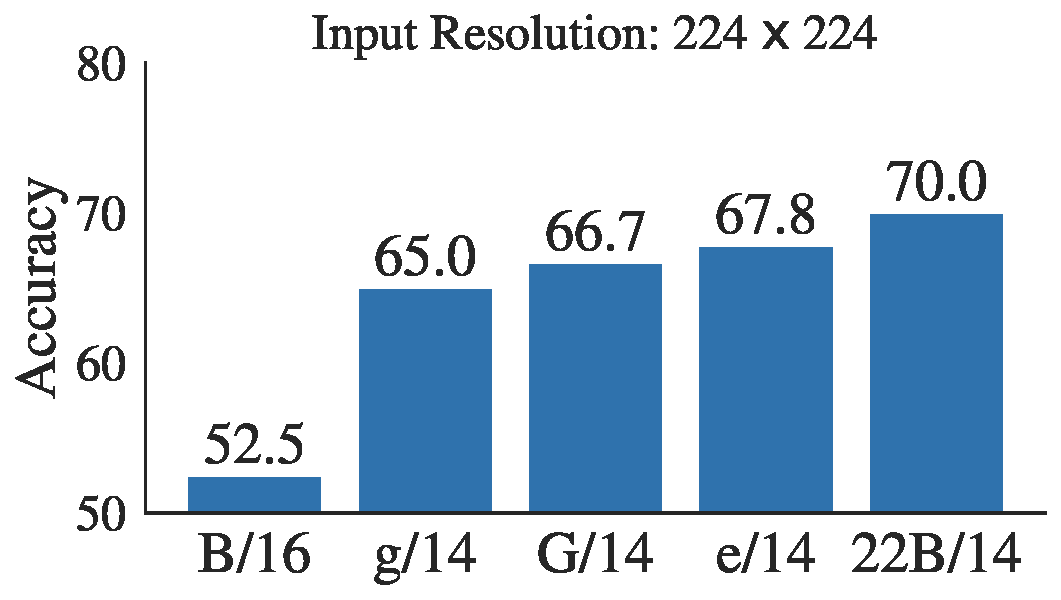
\includegraphics[width=0.35\textwidth]{figs/inat/inat-224.pdf}}
    \hspace{15pt} 
    \subfigure{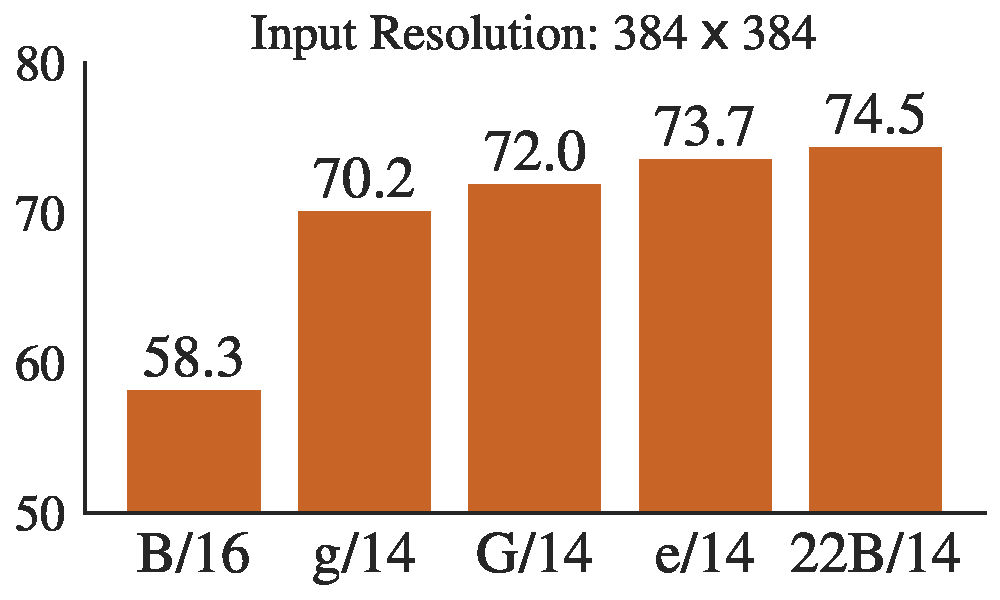
\includegraphics[width=0.35\textwidth]{figs/inat/inat-384.pdf}}
    % \vspace{-5pt}
    \caption{Linear probing on iNaturalist 2017 with different input resolutions. \chonk leads to significant accuracy improvement especially when the input size is small.}
    \label{fig:inat}
    % % \vspace{-10pt}
\end{figure}



We further test linear separability on the fine-grained classification dataset, iNaturalist 2017~\citep{cui2018large}. It has 5,089 find-grained categories, belonging to 13 super-categories. Unlike ImageNet, the image numbers in different categories are not balanced. The long-tail distribution of concepts is more challenging for classification. We compare \chonk with the other ViT variants. 
% For fair comparison, we resize the input images to a fixed size and use those models to extract features for linear classification. 
Similar to the linear probing on ImageNet, we use SGD with 0.001 starting learning rate and no weight decay to optimize the models and train for 30 epochs with cosine learning rate schedule with 3 epochs of linear warm-up. We test both $224$px and $384$px input resolutions. \cref{fig:inat} shows the results. We observe that \chonk significantly improves over the other ViT variants, especially with the standard $224$px input resolution. This suggests the large number of parameters in \chonk are useful for extracting detailed information from the images. 

\subsubsection{Zero-shot via locked-image tuning}
\label{sect::lit}
\paragraph{Experimental setup.}
Following the Locked-image Tuning (LiT)~\citep{lit} protocol, we train a text tower contrastively to match the embeddings produced by the frozen \chonk model.
With this text tower, we can easily perform zero-shot classification and zero-shot retrieval tasks.
We train a text Transformer with the same size as ViT-g~\citep{zhai2022scaling} on the English subset of the WebLI dataset~\citep{chen2022pali} for 1M steps with a 32K batch size.
The images are resized to $288$px, and the text is tokenized to 16 tokens using a SentencePiece~\citep{kudo-richardson-2018-sentencepiece} tokenizer trained on the English C4 dataset.

\paragraph{Results.}
\cref{tab:lit} shows the zero-shot transfer results of \chonk against CLIP~\citep{clip}, ALIGN~\citep{align}, BASIC~\citep{basic}, CoCa~\citep{yu2022coca}, LiT~\citep{lit} with ViT-g~\citep{zhai2022scaling} and ViT-e~\citep{chen2022pali} models. 
The bottom part of \cref{tab:lit} compares three ViT models using the LiT recipe.
On all the ImageNet test sets, \chonk{} achieves either comparable or better results. 
Notably, zero-shot results on the ObjectNet test set is highly correlated with the ViT model size. 
The largest \chonk{} sets the new SOTA on the challenging ObjectNet test set.
\Cref{app:lit} shows zero-shot classification examples on OOD images.


% leader boards:
% - INET: https://paperswithcode.com/sota/zero-shot-transfer-image-classification-on-1
% - INET-V2: https://paperswithcode.com/sota/zero-shot-transfer-image-classification-on-3
% - INET-R: https://paperswithcode.com/sota/zero-shot-transfer-image-classification-on-4
% - INET-A: https://paperswithcode.com/sota/zero-shot-transfer-image-classification-on-5
% - OBJNET: https://paperswithcode.com/sota/zero-shot-transfer-image-classification-on-6
% - INET-REAL: https://paperswithcode.com/sota/zero-shot-transfer-image-classification-on-7
\begin{table}
\centering
\caption{Zero-shot transfer results on ImageNet (variants).}
\resizebox{.5\textwidth}{!}{%
\setlength\tabcolsep{4pt} % default value: 6pt
\begin{tabular}{@{}lcccccc@{}}
 \toprule
 Model & IN & IN-v2 & IN-R & IN-A & ObjNet & ReaL \\
 \midrule
 CLIP & 76.2 & 70.1 & 88.9 & 77.2 & 72.3 & - \\
 ALIGN & 76.4 & 70.1 & 92.2 & 75.8 & 72.2 & - \\
 BASIC & 85.7 & 80.6 & 95.7 & 85.6 & 78.9 & - \\
 CoCa & 86.3 & 80.7 & 96.5 & 90.2 & 82.7 & - \\
 \midrule
 LiT-g/14 & 85.2 & 79.8 & 94.9 & 81.8 & 82.5 & 88.6 \\
 LiT-e/14 & 85.4 & 80.6 & 96.1 & 88.0 & 84.9 & 88.4 \\
 LiT-22B & 85.9 & 80.9 & 96.0 & 90.1 & 87.6 & 88.6 \\
 \bottomrule
\end{tabular}
}
\label{tab:lit}
\end{table}

\subsubsection{Out-of-distribution}
\label{subsec:robustness_ood}
% https://colab.corp.google.com/drive/1kJ1XcIWCDQKKEHf6ef9JkgONvd6pLkk3

% TODO(andstein): remove "22B/14 hot" from table & figure

\paragraph{Experimental setup.} We construct a label-map from JFT to ImageNet, and label-maps from ImageNet to different out-of-distribution datasets, namely ObjectNet~\citep{barbu2019objectnet}, ImageNet-v2~\citep{recht2019imagenet_v2} ImageNet-R~\citep{hendrycks2020imagenet_r}, and ImageNet-A~\citep{hendrycks2021imagenet_a}. ImageNet-R and ImageNet-A use the same 200 label subspace of ImageNet (constructed in such a way that misclassifications would be considered egregious~\citep{hendrycks2021imagenet_a}), while ObjectNet has 313 categories, of which we only consider the 113 ones overlapping with the ImageNet label space. For ObjectNet and ImageNet-A we do an aspect-preserving crop of the central 75\% of the image, for the other datasets we first resize them to a square format and then take a 87.5\% central crop. Image input resolution is 224px for pre-trained checkpoints and 384px, 518px, 560px for models fine-tuned on ImageNet.

\paragraph{Results.} We can confirm results from~\citep{taori2020measuring_robustness,djolonga2021robustness_transferability,kolesnikov2020big} that scaling the model increases out-of-distribution performance in line with the improvements on ImageNet. This holds true for models that have only seen JFT images, and for models fine-tuned on ImageNet. In both cases,  \chonk continues the trend of better OOD performance with larger models (\cref{fig:robustness_objectnet}, \cref{tab:robustness_ood}).
While fine-tuning boosts accuracy on both ImageNet and out-of-distribution datasets, the effective robustness~\citep{andreassen2021effective_robustness} decreases (\cref{fig:robustness_objectnet}).
Even though ImageNet accuracy saturates, we see a significant increase on ObjectNet from ViT-e/14 to \chonk.

\begin{figure}[tbp]
    \centering
    % \vspace{-5pt}
    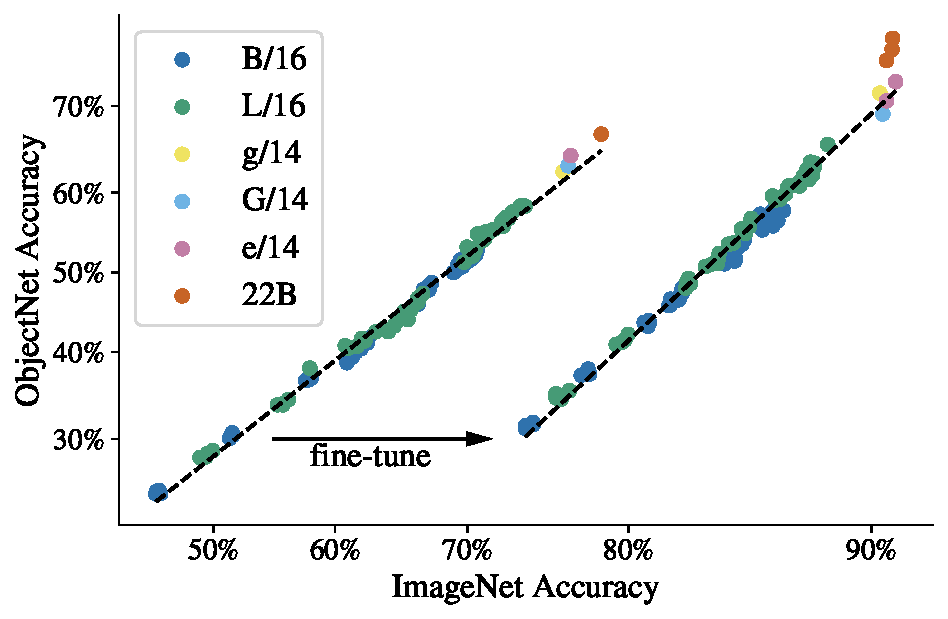
\includegraphics[width=0.6\textwidth]{figs/robustness/objectnet.pdf}
    % \vspace{-5pt}
    \caption{
        OOD classification performance. Axes are log-scaled as proposed in~\citep{taori2020measuring_robustness}. ViT-B and ViT-L are trained on subsets of varying size and varying number of steps on JFT~\citep{zhai2022scaling}. Fine-tuning boosts both ImageNet and ObjectNet performance, but the increase is more pronounced for in-domain data, which decreases effective robustness~\citep{andreassen2021effective_robustness}, visible as a rightwards shift on the plot. Same data as in \cref{tab:robustness_ood}.
    }
    \label{fig:robustness_objectnet}
    % \vspace{-15pt}
\end{figure}
